\documentclass[a4paper, 12pt]{book}
\usepackage[T2A]{fontenc}
\usepackage[utf8]{inputenc}
\usepackage[english, russian]{babel}
\usepackage{upquote}
\usepackage{textcomp}
\usepackage[pdftex]{graphicx}
\graphicspath{{Cover/}}
\usepackage{pdfpages}
\usepackage[pdfborder={0 0 0}]{hyperref}
\usepackage{amsmath}
\usepackage{listings}
\usepackage{epigraph}
%\usepackage{cm-super}
\title{Концепции, Техники и Модели Компьютерного Программирования}
\date{05.06.2003}
\author{ПИТЕР ВАН РОЙ\thanks{Email: pvr@info.ucl.ac.be, Web: http://www.info.ucl.ac.be/\textasciitilde pvr}\\Лувенский католический университет (Лувен-Ла-Нёв)\\Шведский Институт Компьютерных Наук\\ СЕИФ ХАРИДИ\thanks{Email: seif@it.kth.se, Web: http://www.it.kth.se/\textasciitilde seif}\\Лувенский католический университет (Лувен-Ла-Нёв)\\Шведский Институт Компьютерных Наук}

\begin{document}
\lstdefinestyle{customoz}{
  belowcaptionskip=1\baselineskip,
  breaklines=true,
%  frame=L,
  xleftmargin=\parindent,
  language=Oz,
  showstringspaces=false,
  basicstyle=\footnotesize\ttfamily,
  keywordstyle=\bfseries\color{green!40!black},
  commentstyle=\itshape\color{purple!40!black},
  identifierstyle=\color{blue},
  stringstyle=\color{orange},
}

\lstset{language=Oz, mathescape=true, style=customoz}


\renewcommand {\contentsname} {Оглавление}
\renewcommand {\chaptername} {Глава}
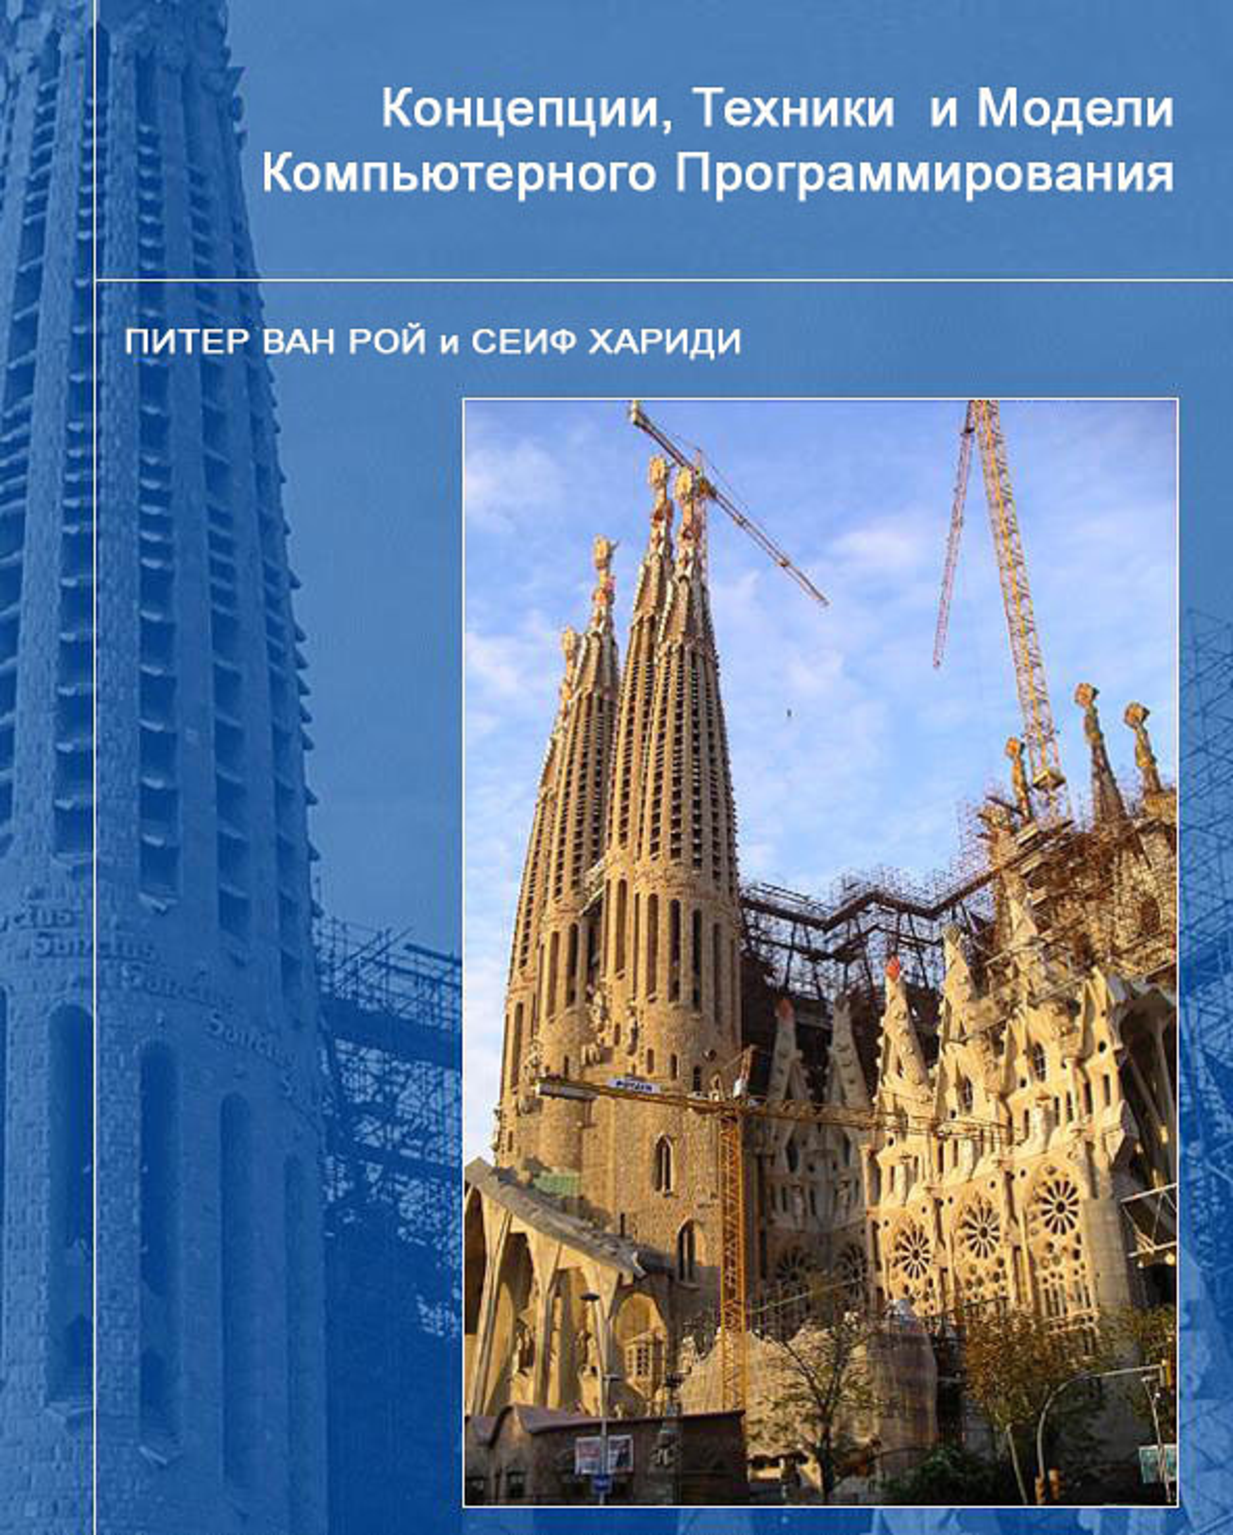
\includepdf{Cover.pdf}

{\let\newpage\relax\maketitle}
\maketitle
\tableofcontents

\chapter*{Предисловие}
\markboth{\MakeUppercase{Предисловие}}{}
\addcontentsline{toc}{chapter}{Предисловие}

{\setlength{\epigraphwidth}{0.8\textwidth} \epigraph{Шесть слепых мудрецов ощупали слона и начали обсуждать свои наблюдения. ``Это замечательно'' сказал первый, ``слон похож на верёвку: тонкий и гибкий.'' ``Нет, нет, не так'' сказал второй, ``слон похож на дерево: прочно стоит в земле.'' ``Изумительно'' сказал третий, ``слон похож на стену.'' ``Невероятно'' сказал четвёртый, ``слон --- это труба заполненная водой.'' ``Что это за странный зверь, который состоит из разных частей'' сказал пятый. ``Действительно странно'' сказал шестой, ``но в основе должна лежать некая гармония. Этот вопрос нужно исследовать подробнее.''}{\emph{---Свободная адаптация классической индийской сказки.}}}

{\setlength{\epigraphwidth}{0.8\textwidth} \epigraph{``Язык программирования подобен естественному, человеческому языку в том плане, что позволяет создавать определённые метафоры, образы и способы мышления.''}{\emph{---``Переворот в сознании: дети, компьютеры и плодотворные идеи'' \cite{141}, Сеймур Пейперт (1980)}}}

Один из подходов в изучении программирования на компьютере --- это изучение языков программирования. Но число языков программирования огромно, настолько огромно, что изучение их всех --- это непрактичное занятие. Что мы можем сделать с этой необъятностью? Мы можем выбрать малое количество языков, представляющих различные программные парадигмы. Но из такого подхода мы мало что сможем извлечь рассматривая программирование как единую дисциплину. Эта книга использует другой подход.

Мы сфокусировались на \emph{концепциях} и \emph{техниках} программирования, а также на их использовании, а не на языках программирования. Концепции представлены в терминах вычислительных моделей. Вычислительная модель --- это формальная система, которая определяет как должны выполняться вычисления. Существует множество способов определения вычислительных моделей. Поскольку эта книга разрабатывалась с учётом на практику, то очень важно чтобы вычислительная модель приносила прямую пользу программисту. Далее мы будем определять её в терминах важных для программистов концепций: типы данных, операции и язык программирования. Термин вычислительная модель уточняет неточное понятие ``парадигмы программирования''. Во всей книге рассказывается о вычислительных моделях, а не парадигмах программирования. Иногда мы будем использовать фразу ``модель программирования''. Это относится к тому, что необходимо программисту: техники программирования и принципы проектирования стали возможны благодаря вычислительным моделям.

Каждая вычислительная модель имеет свой собственный набор техник программирования и подходов к программированию. Число различных полезных вычислительных моделей гораздо меньше чем число языков программирования. Эта книга покрывает много широко известных моделей, также рассмотрены некоторые малоизвестные модели. Главным критерием присутствующих моделей являлась их полезность на практике.

Каждая вычислительная модель основана на простом центральном языке который называется \emph{языком ядра (kernel language)}. Языки ядра вводятся постепенно, добавляя одну концепцию к другой. Это даёт нам возможность показать глубокую взаимосвязь между различными моделями. Часто простое добавление одной новой концепции переворачивает мир в программировании. Например, добавление разрушающих присваиваний (явное состояние) к функциональному программированию даёт нам объектно-ориентированное программирование.

Как мы решаем какую концепцию следует добавить при переходе от одной модели к другой? Мы много раз коснёмся этого вопроса на протяжении этой книги. Главным критерием является \emph{принцип творческого расширения}. Грубо говоря новая концепция добавляется тогда, когда программы становятся сложными из-за технических причин и тем самым отдаляются от решаемых задач. Добавление концепции к языку ядра позволяет сохранять простоту программы, при условии если концепция была выбрана верно. Более подробно это объясняется в Приложении D. Этот принцип лежит в прогрессии языков ядра, представленных в книге.

Приятная особенность в подходе языка ядра в том, что он даёт нам возможность использовать вместе различные модели в одной программе. Обычно это называется \emph{мультипарадигменным программированием}. Это вполне естественно, поскольку означает просто использование нужной концепции для проблемы, вне зависимости от того, из какой вычислительной модели она появилась. Мультипарадигменное программирование --- это старая идея. Например, архитекторы Lisp и Scheme давно придерживаются подобных взглядов. Однако, в этой книге мультипарадигменное программирование применяется более глубже и шире, чем было до сих пор.

С точки зрения моделей вычисления, книга освещает с других углов важные проблемы в информатике. Мы представляем три таких областей, как архитектура графического интерфейса пользователя, надёжное распределённое программирование и программирование в ограничениях. Мы покажем как разумное комбинирование нескольких моделей вычислений может помочь в решении некоторых проблем в этих областях.

\subsection*{Упомянутые языки}

В этой книге мы упомянули много языков программирования и связали их конкретными вычислительными моделями. Например, Java и Smalltalk основаны на объектно-ориентированной модели. {\selectlanguage{english}Haskell} и {\selectlanguage{english} Standard ML} основаны на функциональной модели. Prolog и Mercury основаны на логической модели. Но не все интересные языки можно классифицировать подобным образом. Отметим некоторые языки имеющие свои особенности. Например, Lisp и Scheme пионеры во многих концепциях, представленных здесь. Erlang --- это функциональный, по сути параллельный и поддерживающий отказоустойчивое распределённое программирование язык программирования.

Выделим четыре языка как представителей важных моделей вычислений: Erlang, Haskell, Java и Prolog. Мы идентифицируем вычислительные модели каждого языка в терминах единой системы этой книги. Если вы хотите получить более подробную информацию об этих языках, то обратитесь к соответствующей литературе. В связи с ограниченностью объёма книги мы не можем упомянуть здесь все интересные языки. Отсутствие упоминания в этой книге какого-либо языка ни в коем случае не может служить критерием оценки.

\section*{Цели книги}

\subsection*{Обучение программированию}

Главная цель книги --- научить программированию как единой дисциплине с научной основой, которая будет полезна для практикующего программиста. Рассмотрим ближе что это обозначает.

\subsection*{Что такое программирование?}

Мы определяем \emph{программирование} как общую деятельность человека, обозначающую акт расширения или изменения функциональности системы. Программирование --- это широко распространённая деятельность, выполняемая и не-специалистами (например, потребителями, устанавливающими настройки своего будильника или мобильного телефона) и специалистами (программистов на компьютере, аудитории этой книги).

Эта книга посвящена построению программных систем. С этой точки зрения, программирование --- это шаг между описанием системы и запуском программы, реализующей эту систему. Шаг состоит из проектирования архитектуры программы, абстракций и кодирования их в язык программирования. Это широкое описание, возможно гораздо шире чем обычное значение, вкладываемое в слово ``программирование''. Оно покрывает и ``малое'' программирование и ``большое''. Оно покрывает и (не зависящие от языка) архитектурные вопросы и (зависящие от языка) вопросы кодирования. Оно основывается больше на концепциях и их использовании нежели на каком-либо языке программирования. Мы считаем что это общее описание является естественным для обучения программированию. Оно позволяет взглянуть на многие проблемы абстрагируясь от ограничений любого конкретного языка или методологии проектирования. При использовании в определённых ситуациях, общее описание адаптируется к используемым инструментам, с учётом их возможностей и ограничений.

\subsection*{И наука и технология}

Программирование, как было определено выше, состоит из двух основных частей: технологии и научной основы. Технология состоит из инструментов, практических техник, и стандартов, \emph{позволяющих программировать}. Наука состоит из широкой и глубокой теории, позволяющей \emph{понимать} программирование и моделировать дальнейшее развитие событий. В идеале наука должна описывать технологию наиболее прямым и полезным способом.

Если выбросить хотя бы одну часть, то мы больше не занимаемся программированием. Без технологии мы будем заниматься чистой математикой. Без науки мы становимся ремесленниками, то есть, у нас отсутствует глубокое понимание. Выражаясь корректнее, обучение программированию обозначает и обучение технологии (существующих инструментов) и науке (фундаментальные концепции). Знание инструментов подготавливает студентов к настоящему. Знание концепций подготавливает студентов к будущим разработкам.

\subsection*{Больше чем ремесло}

Несмотря на многие попытки введения научной базы, программированию почти всегда обучают как ремеслу. Обычно обучение велось в контексте одного (или нескольких) языков программирования (например, Java, дополненная Haskell, Scheme или Prolog). Исторические события происходящие при развитии какого-либо конкретно взятого языка тесно переплетаются с фундаментальными концепциями и их нельзя отделить друг от друга. Возникает путаница между инструментами и концепциями. Что более важно различные школы программирования основываются на различных видениях программирования, называемых ``парадигмами'': объектно-ориентированное, логическое, функциональное и т.д. Каждая школа обучает своей собственной науке. Программирование было потеряно как единая дисциплина.

Обучение программированию в таком стиле подобно различным школам строительства мостов: одна школа обучает строительству деревянных мостов, а другая школа учит строительству железных мостов. Выпускники подобных школ невольно рассматривают ограничения налагаемые деревом или железом как фундаментальные и не думают об использовании дерева и железа вместе.

В результате программы страдают от бедной архитектуры. Мы даём примеры на основе Java, но подобная проблема существует во всех языках в разной степени. Параллелизм в Java сложен для использования и дорог в плане вычислительных ресурсов. Из-за этих трудностей, программисты обученные на Java делают вывод что параллелизм - это фундаментально сложная и дорогостоящая концепция. Спецификации программ строятся вокруг сложностей, и часто в искажённом виде. Но эти трудности вообще не фундаментальны. Существуют формы параллелизма, которые являются очень полезными и лёгкими в программировании в виде последовательных программ (например, потоковое программирование, на примере Unix pipe). Кроме того, возможно реализовать нити, базовую единицу параллелизма, почти такие же дешёвые, как и вызов процедуры. Если программиста обучили параллелизму правильным способом, то он или она может определять что ему нужно и программировать в системах без ограничений на параллелизм (включая улучшенные версии Java).

\subsection*{Подход язык ядра}

Практические языки программирования масштабируются до программ, состоящих из миллионов строк кода. Они предоставляют богатый набор абстракций и синтаксиса. Как мы можем отделить фундаментальные концепции языка, лежащие в основе их успеха, от исторических событий? Подход язык ядра показывает этот способ. Согласно этому подходу практические языки транслируются в \emph{язык ядра}, который состоит из малого числа \emph{программно-значимых} элементов. Богатый набор абстракций и синтаксиса зашифрован в этом малом языке ядра. Этот подход даёт и программисту и студенту возможность понять то, что выполняет язык. Язык ядра даёт простую формальную семантику, которая позволяет производить рассуждения о корректности программ и их сложности. Что в свою очередь даёт прочный фундамент для программистской интуиции и программных техниках строящихся поверх неё.

Большое разнообразие языков и парадигм программирования может быть смоделировано малым набором языков ядра, находящихся в близком родстве. Отсюда следует что подход языка ядра является по настоящему языко-независимым способом обучения программированию. Поскольку любой язык транслируется в язык ядра, являющийся подмножеством более большего, более полного языка ядра, то восстанавливается единство программирования.

Упрощение сложного явления на более простые составные части --- характерно для научного метода. Этот результативный подход используется во всех науках. С помощью такого подхода можно достичь глубокого понимания явлений, и этим достигается возможность предсказывать события. Например, с помощью науки мы можем проектировать \emph{любые} мосты (сделанные из дерева, железа, других материалов или из их сочетаний) и предсказывать их поведение в терминах более простых концепций, таких как сила, энергия, напряжение, и других законов \cite{62}.

\subsection*{Сравнение с другими подходами}

Сравним подход язык ядра с тремя другими способами преподавания прочного и широкого научного фундамента программирования:

\begin{itemize}
\item{\emph{Основополагающие исчисления}, такие как $\lambda$ исчисление или $\pi$ исчисление, упрощают программирование до минимального набора элементов. Эти элементы выбраны так, чтобы упростить математический анализ и в этом случае они не помогают программистской интуиции. Они очень удобны для теоретиков, но не всегда полезны для практикующих программистов. Основополагающие исчисления удобны для обучения фундаментальным основам и ограничениям программирования на компьютере, но малопригодны для написания приложений в целом.}

\item{\emph{Виртуальная машина} определяет программирование в терминах реализации на идеализированной машине. Виртуальная машина даёт некую разновидность операционных семантик с концепциями, родственными физическому оборудованию реального компьютера. Это полезно для проектирования компьютеров, реализации языков или выполнения симуляций. Но не пригодно для рассмотрения программ и их абстракций.}

\item{\emph{Мультипарадигменные языки} --- это языки, вобравшие в себя несколько программных парадигм. Например, Scheme --- это и функциональный и императивный (\cite{38}) язык, а Leda имеет элементы функционального, объектно-ориентированного и логического (\cite{27}) языка. Полезность мультипарадигменного языка зависит от того насколько в него интегрированы различные парадигмы.}
\end{itemize}

Подход язык ядра комбинирует в себе все элементы этих подходов. Хорошо спроектированный язык ядра покрывает большое количество концепций, также, как и хорошо спроектированный мультипарадигменный язык. Если концепции независимы, то язык ядра может быть представлен как простая формальная семантика, такие как фундаментальные исчисления. И наконец формальные семантики могут быть виртуальными машинами высокоуровневых абстракций. Что в свою очередь облегчает программистам процесс рассматривания программ.

\subsection*{Проектирование абстракций}

Вторая цель этой книги --- это обучение проектированию программных абстракций. Наиболее тяжёлая работа программиста, и также наиболее вознаграждаемая, --- это не написание программ, но \emph{проектирование абстракций}. Программирование на компьютере это, в основном, проектирование и использование абстракций для достижения новых целей. Наше вольное определение \emph{абстракции}: абстракция --- это инструмент или устройство для решения определённой проблемы. Обычно одна абстракция может быть использована для решения многих других проблем. Эта универсальность --- одна из ключевых особенностей абстракций.

Абстракции --- это настолько важная часть нашей жизни, что часто мы забываем о них. Некоторыми типичными абстракциями являются книги, кресла, отвёртки и автомобили.\footnote{Также абстракциями могут быть карандаши, гайки, болты, провода, транзисторы, корпорации, песни и дифференциальные уравнения. Абстракции --- это не обязательно материальные объекты.} Абстракции можно классифицировать по иерархии специализации (например, ``карандаш'' --- это более специализированная версия ``инструмент для письма'', но они оба являются абстракциями).

Внутри компьютерных систем количество абстракций достигает особенно больших чисел. Современные компьютеры --- это очень сложные системы, состоящие из оборудования, операционной системы, промежуточных прикладных программ и программных уровней, каждая из которых основывается на работе тысяч людей на протяжении многих десятилетий. Они содержат огромное число абстракций, которые работают вместе очень точно организованным способом.

Проектирование абстракций --- это не всегда лёгкое занятие. Этот процесс может быть долгим и болезненным, и заключается в испытании различных подходов, их отбраковке и улучшении. Но результат очень значим. Не будет большим преувеличением сказать что цивилизация построена на удачных абстракциях \cite{134}. Новые абстракции разрабатываются каждый день. Некоторые старинные абстракции, такие как колесо и арка, всё ещё с нами. Некоторые современные абстракции, такие как мобильный телефон, быстро стали частью нашей повседневной жизни.

Для достижения второй цели мы следуем такому подходу. Мы начинаем с концепций программирования, являющихся сырым материалом для строительства абстракций. Мы вводим большое количество известных на сегодня концепций, в частности лексическая область видимости, высокоуровневое программирование, композиционность, инкапсуляция, параллелизм, исключения, ленивое выполнение, безопасность, явное состояние, наследование и недетерминированный выбор. Для каждой концепции мы даём техники построения абстракций. Мы даём большое количество примеров для последовательных, параллельных и распределённых абстракций. Мы даём некоторые общие законы построения абстракций. Многие из этих законов имеют свои аналоги в других прикладных науках, поэтому, такие книги как \cite{69}, \cite{55} и \cite{62} могут быть источником вдохновения для программистов.

\section*{Главные особенности}

\subsection*{Педагогический подход}

Существует два взаимодополняющих подхода обучения программированию как строгой дисциплины:

\begin{itemize}
\item{\emph{Подход, основанный на вычислениях}, представляет программирование как способ определения операций на машинах. Он основан на представлениях студента о реальном мире и исполнения операций на настоящих системах. Этот подход особенно эффективен на интерактивных системах: студент может создавать фрагменты программы и сразу же увидеть как они работают. Сокращение времени между размышлениями в стиле ``что если'' и получением результата особенно полезны для понимания. При этом мы не теряем точность, поскольку формальную семантику программы можно задавать в терминах абстрактной машины.}

\item{\emph{Подход основанный на логике} представляет программирование как ответвление от математической логики. Логика ничего не говорит об исполнении, но обращает внимание на свойства программ, являющихся высокоуровневыми абстракциями. Программы являются математическими конструкциями, подчиняющимися логическим законам. Рассуждения основываются на логических законах. Подход основанный на логике более труден для студентов в плане понимания, но этот подход необходим для точных описаний того, что делает программа.}
\end{itemize}

Как и \emph{Структура и Интерпретация Компьютерных Программ} за авторством Абельсона, Сассмана и Сассмана (Structure and Interpretation of Computer Programs, by Abelson, Sussman, \& Sussman) \cite{1, 2}, наша книга в основном использует подход основанный на вычислении. Концепции иллюстрируются с помощью программных фрагментов, которые можно запускать на сопутствующем программном пакете Системе Программирования Моцарт \cite{129}. Программы конструируются в стиле строительных блоков, из которых составляются базовые концепции, позволяющие в свою очередь создавать более сложные концепции. Последние главы содержат немного логических рассуждений, использующихся для определения спецификаций и использование инвариантов для рассуждения о программах с состояниями.

\section*{Используемые формализмы}

Книга использует единый формализм для представления всех вычислительных моделей и программ, а именно язык Oz и его вычислительная модель. Если более точно, вычислительные модели этой книги --- это тщательно отобранное подмножество Oz. Почему мы выбрали Oz? Главная причина --- это хорошая поддержка подхода языка ядра. Другая причина --- это существование Системы Программирования Mozart.

\section*{Обзор вычислительных моделей}

Эта книга представляет широкий обзор наиболее полезных вычислительных моделей. Модели спроектированы не только с учётом простоты (хотя это тоже важно), но и с учётом того, как программист сможет выразить себя в этих моделях. Кроме того обсуждаются и сами модели. Существует множество различных практических вычислительных моделей, с различными уровнями выразительности, различными программными техниками и различными способами размышлений в рамках конкретно взятой модели. Мы обнаружили что каждая модель обладает своей областью применения. Эта книга объясняет большое количество этих моделей, как они взаимосвязаны друг с другом, как в них программировать и как их комбинировать для того, чтобы получить максимум преимуществ.

\subsection*{Больше --- это не лучше (или хуже), --- это по-другому}

Все модели вычислений имеют свои места. И высказывание о том, что модели с большим числом концепций лучше или хуже --- неправда. А всё потому, что новая концепция подобна обоюдоострому мечу. Добавление концепции в модель вычисления приводит к возникновению новых форм выражений, при этом некоторые программы упрощаются, но одновременно усложняются рассуждения о программах. Например, добавив \emph{явное состояние} (изменяемые переменные) в функциональную модель мы можем выразить все вариации объектно-ориентированных техник программирования. Однако, рассуждения об объектно-ориентированных программах становятся более сложными по сравнению с рассуждениями о функциональных программах. Функциональное программирование --- это вычисление значений с помощью математических функций. С течением времени ни функции, ни значения не изменяются. Явное состояние --- это один из способов моделирования явлений, изменяющихся с течением времени: получается некий контейнер, содержимое которого может обновляться. Большая мощь этой концепции усложняет рассуждения о ней.

\subsection*{Важность совместного использования моделей}

Изначально каждая модель вычисления была спроектирована для изолированного использования. Соответственно использование нескольких различных моделей в одной программе может показаться отклонением. Мы считаем что это не так. Но модели это не просто монолитные блоки не имеющие между собой ничего общего, напротив, у разных моделей есть много общего. Например, разница между декларативными и императивными моделями, параллельными и последовательными моделями, по сравнению с их общими чертами оказывается весьма малой. По этой причине, совместное использование моделей не такая сложная задача.

Но даже если это технически возможно, зачем \emph{нужно} использовать несколько моделей в одной программе? Ответ на этот вопрос простой: мы не программируем моделями, но программируем концепциями и способами их комбинации. В зависимости от используемой концепции можно рассматривать программирование как некоторую конкретную модель. Модель проявляется как некоторая разновидность вторичного явления. Некоторые аспекты упрощаются, другие усложняются и рассуждения о программах ведутся определённым способом. Для хорошо написанной программы использование различных моделей --- это вполне естественное явление. На данном начальном этапе такой ответ может показаться весьма загадочным. Но позже всё станет ясно.

Важным принципом, красной нитью проходящим через всю книгу, является использование концепций, традиционно ассоциируемых с одной моделью, в других более общих моделях с целью получения более выраженного эффекта. Например, концепции лексической области видимости и высокоуровневого программирования, обычно ассоциируемые с функциональным программированием, полезны во всех моделях. Это явление хорошо известно в сообществе функциональных программистов. Функциональные языки уже давно расширяются с помощью явного состояния (например Scheme \cite{38} и Standard ML \cite{126, 192}) а в последнее время и с помощью параллелизма (например, Concurrent ML \cite{158} и Concurrent Haskell \cite{149, 147}).

\subsection*{Ограничения единственной модели}

Мы выяснили что хороший стиль программирования требует использования концепций программирования, которые обычно ассоциированы с различными моделями вычислений. Языки, реализующие только одну вычислительную модель сталкиваются со следующими трудностями:

\begin{itemize}
\item{Объектно-ориентированные языки поощряют чрезмерное использование состояния и наследования. Объекты, по-умолчанию, обладают состоянием. И хотя такой подход кажется простым и интуитивно понятным, на самом деле программирование усложняется, например, возникают трудности с параллелизмом (смотрите Раздел 8.2). Шаблоны проектирования, которые определяют общую терминологию для определения хороших техник программирования, обычно описываются в терминах наследования \cite{58}. Во многих случаях вполне достаточно использовать более простые высокоуровневые техники программирования (смотрите Раздел 7.4.7). К тому же наследованием часто злоупотребляют. Например, в объектно-ориентированных графических интерфейсах пользователя часто рекомендуется использовать наследования для расширения общих классов виджетов функциональностью, зависящей от приложения (например, компоненты Swing для Java). Это противоречит методу разделения проблемы на составные части.}

\item{Функциональные языки поощряют чрезмерное использование высокоуровневого программирования. Типичные примеры это монады и каррирование. Монады используются для кодирования состояния через всю программу. Такой подход усложняет программы, но не позволяет достичь модульности настоящего явного состояния (смотрите Раздел 4.7). Каррирование позволяет частично применять функцию передав ей только некоторые аргументы. В результате возвращается новая функция, которая ожидает ввода остальных аргументов. Тело функции не будет выполняться до тех пор, пока функции не будут переданы все аргументы. Оборотной стороной является трудность ответа на вопрос ``Получила ли функция все аргументы или она по-прежнему каррирована?'' (``ожидает'' остальные аргументы).}

\item{Логические языки, такие как Prolog, поощряют чрезмерное использование синтаксиса дизъюнктов Хорна и запросов. Эти языки определяют все программы как коллекции дизъюнктов Хорна, напоминающие простые логические аксиомы в стиле ``if-then''. В результате многие алгоритмы оказываются обфусцированными, будучи написанными в таком стиле. К тому же всегда необходимо использовать запросы, даже если они не нужны (смотрите \cite{196}).}
\end{itemize}

Эти примеры в известной степени субъективны; трудно быть полностью объективным в отношении хорошего стиля программирования и выразительности языка. Поэтому нельзя судить о моделях основываясь на этих высказываниях. Скорее эти слова служат намёком на то, что никакая модель сама по себе не может быть панацеей от всех проблем. Каждая модель в чём-то лучше, но и в то же время в чём-то хуже. Эта книга пытается показать сбалансированный подход, иногда будет использоваться какая-либо изолированная единственная модель, а иногда будут использоваться сразу несколько моделей если их применение целесообразно.

\section*{Обучение по книге}

Мы объясним как эта книга соотносится с учебной программой по информатике и в обучении каких курсов её можно использовать. Под \emph{информатикой (informatics)} мы имеем в виду весь диапазон информационных технологий, включая компьютерные науки (computer science), разработку компьютеров и информационные системы. Информатику иногда называют \emph{вычислением (computing)}.

\subsection*{Роль в учебной программе по информатике}

Рассмотрим дисциплину программирования независимо от любой другой области информатики. По нашему опыту она естественным образом делится на три основные темы: 

\begin{enumerate}
\item{Концепции и техники.}

\item{Алгоритмы и структуры данных.}

\item{Архитектура программ и разработка программного обеспечения.}
\end{enumerate}

В этой книге дано подробное рассмотрение темы (1) и введение в (2) и (3). В каком порядке должны преподаваться темы? Между темами (1) и (3) существует сильная взаимная зависимость. Опыт показывает что разработка архитектуры программ должна преподаваться как можно раньше, таким образом студенты избегут приобретения плохих привычек. Однако это только одна часть целой истории, поскольку студенты должны знать о концепциях, для того, чтобы суметь выразить их архитектуры. Парнас использует подход, который начинается с темы (3) и применяет императивную вычислительную модель \cite{143}. Поскольку эта книга использует много вычислительных моделей, то мы рекомендуем использовать её для параллельного обучения темам (1) и (3), постепенно вводя новые концепции и принципы проектирования. В программе информатики в Лувенском католическом университете (UCL), мы отводим восемь семестро-часов для каждой темы. Сюда входят лекции и лабораторные занятия. Все три темы вместе дают одну шестую полного учебного курса по информатике для дипломников и инженерных направлений обучения.

Есть ещё один момент, на который мы хотели бы обратить ваше внимание: обучение параллельному программированию. В традиционных учебных планах по информатике параллелизм преподаётся через расширение модели с состоянием, также как Глава 8 расширяет Главу 6. Такой подход по праву считается сложным и трудным для программирования. Существуют другие, более простые формы параллельного программирования. Декларативный параллелизм Главы 4 гораздо проще для программирования и часто может быть использован вместо параллелизма на состояниях (смотрите цитату, которой начинается Глава 4). Потоковому параллелизму, простой форме декларативного параллелизма, --- обучают первокурсников в Массачусетском технологическом институте (MIT) и других учебных заведениях. Другой простой форме параллелизма --- передаче сообщений между нитями --- посвящена Глава 5. Мы полагаем что декларативный параллелизм и параллелизм на передаче сообщений являются частью стандартного учебного плана и должны преподаваться до параллелизма на состояниях.

\subsection*{Курсы}

Мы использовали эту книгу в качестве учебного пособия для нескольких курсов начиная с второкурсников и заканчивая выпускниками \cite{200, 199, 157}. В текущей форме эта книга \emph{не} может быть использована в роли первого курса обучения программированию, но используемые подходы могут быть адаптированы для таких целей.\footnote{Мы будем рады помочь любому кто решит провести такую адаптацию.} Студенты уже должны обладать некоторым опытом программирования (например, практическое введение в программирование и знание простых структур данных, таких как последовательности, наборы, стеки, деревья и графы) и некоторой математической зрелостью (например, начальный курс анализа, дискретной математики или алгебры). Книга содержит много материала, по крайней мере четыре семестра-часов лекций и много лабораторных работ. Вот некоторые курсы в которых может применяться материал из этой книги:

\begin{itemize}
\item{Курс по концепциям и техникам программирования для студентов бакалавриата. В качестве вводного материала следует использовать Главу 1. Продолжение курса в Главах 2-8. В зависимости от глубины изучения материала, можно сделать акценты на алгоритмах (для обучения алгоритмам вместе с программированием), параллелизму (при желании можно не изучать) или формальным семантикам (для развития интуиции).}

\item{Курс по прикладным моделям программирования для студентов бакалавриата. Сюда входят: реляционное программирование (Глава 9), специфичные языки программирования (особенно {\selectlanguage{english}Erlang}, {\selectlanguage{english}Has\-kell}, {\selectlanguage{english}Java} и {\selectlanguage{english}Prolog}), программирование графического интерфейса пользователя (Глава 10), распределённое программирование (Глава 11) и программирование в ограничениях (Глава 12). Этот курс --- естественное продолжение предыдущего курса.}

\item{Курс по параллельному и распределённому программированию для студентов бакалавриата (Главы 4, 5, 8 и 11). Студенты уже должны обладать некоторым опытом в программировании. Курс можно начинать с некоторых частей Глав 2, 3, 6 и 7 для введения в декларативное программирование и программирование с состоянием.}

\item{Курс по моделям вычислений для магистров (вся книга, включая семантики в Главе 13). В данном курсе основной акцент можно поставить на взаимосвязях между моделями и их семантикой.}
\end{itemize}

На web сайте книги содержится больше информации о курсах, включая слайды и лабораторные задания для некоторых из них. На web сайте есть анимированный интерпретатор, выполненный Кристианом Шальтом (Christian Schulte), показывающий как выполняются языки ядра в семантике абстрактной машины. Книга может быть использована в качестве дополнения к другим курсам:

\begin{itemize}
\item{Часть курса о программировании в ограничениях для студентов бакалавриата (Главы 4, 9 и 12).}

\item{Часть курса об интеллектуальных взаимодействующих приложениях для магистрантов (некоторые части из всей книги, следует уделить особое внимание Части III). При желании книга может быть дополнена материалами по искусственному интеллекту (например, \cite{160}) или по многоагентным системам (например, \cite{205}).}

\item{Часть курса о семантиках для студентов бакалавриата. Все модели формально определены в тех главах, в которых они встречаются, но в Главе 13 основное внимание уделено семантикам. С помощью Главы 13 мы даём полную картину для определения семантик завершённого современного языка программирования.}
\end{itemize}

В этой книге помимо прочной теоретической базы уделено внимание и к \emph{практическому} преподаванию тем. В каждой главе содержатся множество программных фрагментов, каждую из которых можно запустить в системе Моцарт (смотрите ниже). Благодаря этим фрагментам, лекции курсов обретают живую интерактивную демонстрацию концепций. Мы обнаружили что студенты очень высоко оценивают подобный стиль проведения лекций.

Каждая глава заканчивается набором задач, в которые обычно входит программирование. Они могут решаться в системе Моцарт. Для наиболее лучшего усвоения материала глав мы рекомендуем студентам решать столько задач сколько это возможно. Решение упражнений, помеченных как (\emph{сложная задача}) могут занять от нескольких дней до нескольких недель. Упражнения помеченные как (\emph{исследовательский проект}) являются нерешёнными и их решение может привести к значительному вкладу в исследование задачи.

\subsection*{Программное обеспечение}

Полезной особенностью книги является то, что все фрагменты программ можно запустить на программной платформе \emph{Система Программирования Моцарт}. Моцарт --- это полнофункциональная система программирования промышленного уровня поставляемая с интерактивной, инкрементальной средой разработки и полным набором инструментов. Производится компиляция в эффективный платформно-независимый байткод, запускающийся на многих вариациях Unix, Windows и Mac OS X. Распределённые программы могут запускаться на всех вышеперечисленных системах. На web сайте Моцарт, \verb|http://www.mozart-oz.org|, содержится наиболее полная информация, включающая в себя бинарные файлы доступные для скачивания, документацию, научные публикации, исходные коды и списки рассылки.

Все вычислительные модели упомянутые в этой книге эффективно реализуются системой Моцарт. Такой подход идеален для совместного использования моделей в одной программе и для сравнивания моделей с помощью написания программ, решающих задачу в различных моделях. Поскольку каждая модель реализована эффективно, то все программы могут быть написаны в единственной модели. При необходимости в педагогически оправданных случаях можно вводить другие модели. Например, программы могут быть полностью написаны в объектно-ориентированном стиле, дополненном в нужных местах небольшими декларативными добавлениями.

Система Моцарт --- это результат долгой разработки Консорциума Моцарт, плод совместных неформальных исследований и разработок трёх лабораторий. Разработка началась с 1991 года. Система выпускается со всеми исходными кодами под лицензионным соглашением Open Source. Первый публичный релиз был выпущен в 1995 году. Первый публичный релиз с поддержкой дистрибутива был выпущен в 1999 году. Книга основана на идеальной реализации, наиболее близкой к Моцарт версии 1.3.0, выпущенной в 2003 году. Различия между идеальной реализацией и Моцартом перечислены на Web сайте книги.

\section*{История и благодарности}

Идеи этой книги вынашивались отнюдь не легко. На разработку было затрачено более десяти лет обсуждений, программирования, вычислений, отбрасывания плохих и нахождение хороших и выглядящих хорошими идей. Эта книга --- результат работы многих людей, они вложили сюда свои идеи, реализации, инструменты и приложения. Нам повезло и все мы, включая наших коллег, оказались единомышленниками на протяжении такого долгого периода. Благодаря этому мы оказались в состоянии идти вперёд.

Нашим основным исследовательским инструментом и ``тестовым полигоном'' новых идей была система Моцарт, реализующая язык Oz. Главные архитекторы и разработчики (в алфавитном порядке): Пер Бранд (Per Brand), Торстен Брунклаус (Thorsten Brunklaus), Денис Дачер (Denys Duchier), Донатиен Гролю (Donatien Grolaux), Сеиф Хариди (Seif Haridi), Драган Ховелка (Dragan Havelka), Мартин Хенз (Martin Henz), Эрик Клинтског (Erik Klintskog), Леиф Корнштадт (Leif Kornstaedt), Михаель Мейль (Michael Mehl), Мартин Мюллер (Martin Müller), Тобиас Мюллер (Tobias Müller), Анна Нейдеруд (Anna Neiderud), Константин Попов (Konstantin Popov), Ральф Шайдхаур (Ralf Scheidhauer), Кристиан Шульт (Christian Schulte), Герт Смолка (Gert Smolka), Питер Ван Рой (Peter Van Roy) и Йорг Вюрц (Jörg Würtz). Важный вклад внесли (в алфавитном порядке): Илиез Алоини (Iliès Alouini), Торстен Брунклаус (Thorsten Brunklaus), Рафаэль Коллет (Raphaёl Collet), Фрей Дрейхаммер (Frej Drejhammer), Самех Эль-Ансари (Sameh El-Ansary), Нилс Франсен (Nils Franz{\'e}n), Кевин Глин ({\selectlanguage{english}Glynn Kevin}), Мартин Хомик (Martin Homik), Саймон Линдблом (Simon Lindblom), Бенджамин Лоренц ({\selectlanguage{english}Benjamin Lorenz}), Валентин Месарос (Valentin Mesaros) и Андреас Саймон (Andreas Simon).

Мы выражаем благодарность следующим исследователям и людям, косвенно оказавшим помощь при работе над книгой: Хассан Аит-Качи (Hassan A{\"\i}t-Kaci), Джо Армстронг (Joe Armstrong), Йоахим Дарчхольц (Joachim Durchholz), Андреас Франк (Andreas Franke), Клэр Гардент ({\selectlanguage{english}Claire Gardent}), Фредрик Холмгрен (Fredrik Holmgren), Сверкер Дженсон (Sverker Janson), Торбьёрн Ладжер (Torbj{\"o}rn Lager), Эли Милгром (Elie Milgrom), Йохан Монтелиус (Johan Montelius), Аль-Метуолли Мостафа (Al-Metwally Mostafa), Йоахим Нирен (Joachim Niehren), Лак Онана (Luc Onana), Марк-Антуан Пиерент (Marc-Antoine Parent), Дэйв Парнас (Dave Parnas), Матиас Пайкер (Mathias Picker), Андреас Поделски (Andreas Podelski), Кристоф Понсард (Christophe Ponsard), Махмуд Рафи (Mahmoud Rafea), Юрис Реинфилдс (Juris Reinfelds), Томас Съёланд (Thomas Sj{\"o}land), Фред Спайссенс (Fred Spiessens), Джо Тёрнер (Joe Turner) и Джин Вандердонкт (Jean Vanderdonckt).

Мы выражаем отдельную благодарность людям, помогавшим нам при работе над материалом этой книги. Мы благодарим Рафаэля Коллета ({\selectlanguage{english}Ra\-pha\-\"el Col\-let}) за соавторство Главы 12 и 13 и его работу над практической частью LINF1251, курса, преподаваемого в Лувенском католическом университете (UCL). Мы благодарим Донатиена Гролю (Donatien Grolaux) за три обучающих примера Графического Интерфейса Пользователя (GUI) (использованные в Разделах 10.3.2 - 10.3.4). Мы благодарим Кевина Глинна (Kevin Glynn), написавшего введение в Haskell (Раздел 4.8). Мы благодарим Фрея Дрейхаммера (Frej Drejhammer), Самеха Эль-Ансари (Sameh El-Ansary) и Драгана Ховелка (Dragan Havelka) за работу над практической частью DatalogiII, курса, преподаваемого в Королевском Технологическом Институте (KTH). Мы благодарим Кристиана Шульта (Christian Schulte), ответственного за полное переосмысление и переработку следующей редакции DatalogiII и его комментарии по книге. Мы благодарим Али Одси (Ali Ghodsi), Йохана Монтелиуса (Johan Montelius) и остальных трёх ассистентов за работу над практической частью этой редакции. Мы благодарим Луиса Куесада (Luis Quesada) и Кевина Глинна (Kevin Glynn) за работу над практической частью INGI2131, курса, преподаваемого в Лувенском католическом университете (UCL). Мы благодарим Бруно Картона (Bruno Carton), Рафаэля Коллета (Raphaёl Collet), Кевина Глинна (Kevin Glynn), Донатиена Гролю (Donatien Grolaux), Стефано Гуаланди (Stefano Gualandi), Валентина Месароса (Valentin Mesaros), Аль-Метуолли Мостафу (Al-Metwally Mostafa), Луиса Куесада (Luis Quesada) и Фреда Спайссенса (Fred Spiessens) за корректуру и тестирование примеров программ. И наконец мы благодарны членам Отдела Компьютерных Наук и Инженерии Лувенского католического университета (UCL), Шведского Института Компьютерных Наук и Отдела Микроэлектроники и Информационных Технологий Королевского Технологического Института (KTH). Приносим свои извинения всем, кого мы забыли упомянуть.

Как же нам удалось сохранить результат в простоте работая с такой большой командой разработчиков? Здесь нет никакого чуда, а есть результат чёткого видения цели и аккуратно спроектированной методологии на разработку и полировку которых ушло более десяти лет (итоги смотрите в \cite{196}; кратко резюмируя можно сказать следующее: ``архитектура бывает либо простой, либо неправильной''). Примерно в 1990 году некоторые из нас, обладающих сильными знаниями в построении систем и прочной теоретической базой, объединились и инициировали проект ACCLAIM спонсором которого выступил Европейский Союз (1991 --- 1994). По некоторым причинам этот проект стал центральным. Среди многих других трудов значимыми вехами стали три работы: Сверкер Дженсон (Sverker Janson) и Сеиф Хариди (Seif Haridi) в 1991 \cite{93} (множественные парадигмы в AKL), Герт Смолка (Gert Smolka) в 1995 \cite{180} (построение абстракций в Oz) и Сеиф Хариди (Seif Haridi) и другие в 1998 \cite{72} (надёжное открытое распределение в Oz). Первая публикация об Oz была опубликована в 1993 году и уже тогда содержала много важных идей \cite{80}. После ACCLAIM две лаборатории продолжили совместную работу над идеями Oz: Programming Systems Lab --- Лаборатория Программируемых Систем (DFKI, Universit{\"a}t des Saarlandes --- Саарский Университет и Collaborative Research Center --- Совместный Научно-Исследовательский Центр SFB 378) в Саарбрюкене, Германия и Intelligent Systems Laboratory --- Лаборатория Интеллектуальных Систем (Swedish Institute of Computer Science --- Шведский Институт Компьютерных Наук) в Стокгольме, Швеция.

Первоначально язык Oz был разработан Гертом Смолка (Gert Smolka) в Programming Systems Lab \cite{79, 173, 179, 81, 180, 74, 172}. Хорошая архитектура языка и высокое качество его реализации были созданы во многом под руководством Герта Смолка (Gert Smolka) и высоким профессионализмом лаборатории в области построения систем. Среди разработчиков мы должны отметить Кристиана Шульта (Christian Schulte) и его роль в общей координации разработки, Дениса Дачера (Denys Duchier) за его активную поддержку пользователей и Пера Бранда (Per Brand) за его роль в координировании разработки реализации распределённости. В 1996 году Германские и Шведские лаборатории присоединились к Отделу Компьютерных Наук и Инженерии (Department of Computing Science and Engineering, Лувенского католического университета - UCL), в Лувен-ла-Нёв, Бельгия, когда первый автор переехал в Лувен-ла-Нёв. Вместе три лаборатории сформировали Консорциум Моцарт (Mozart Consortium) с нейтральным Web сайтом \verb|http://www.mozart-oz.org|, таким образом проводимая работа не привязана к одному институту.

При создании книги использовался \LaTeXe, flex, xfig, xv, vi/vim, emacs и Mozart. Изначально использовался компьютер Dell Latitude с Red Hat Linux и KDE, а затем Apple Macintosh PowerBook G4 с Mac OS X и X11. Первый автор благодарит Валлонский регион Бельгии за их щедрую поддержку во время работы над Oz/Mozart в Лувенском католическом университете в проекте PIRATES.

\section*{Чего здесь нет}

Есть две главные темы, отсутствующие в книге:

\begin{itemize}
\item{\emph{Статическая типизация}. Использованный формализм этой книги --- динамическая типизация. Несмотря на достоинства статической типизации для проверки программ, безопасности и эффективности реализации, мы её едва упомянули. Причина в том, что эта книга фокусируется на выражении вычислений с концепциями программирования, с как можно меньшим числом ограничений. У нас и так есть много тем, которые нужно рассказать в лимитированном объёме книги, и свидетельство тому --- размер книги.}

\item{\emph{Специализированные техники программирования}. Множество техник программирования слишком обширно для их охвата в рамках одной книги. В дополнение к общим техникам, описанным в этой книге, каждая предметная область какой-либо проблемы имеет свою особую технику. В этой книге охвачены не все техники; попытка охватить все техники приведёт к удвоению или к утроению размера. Для восполнения этого недостатка мы отошлём читателя к некоторым хорошим книгам, в которых рассматриваются предметные области некоторых проблем: техники искусственного интеллекта \cite{160, 136}, алгоритмов \cite{41}, объектно-ориентированных шаблонов программирования \cite{58}, мультиагентное программирование \cite{205}, базы данных \cite{42} и численные методы \cite{153}.}
\end{itemize}

\section*{Последние комментарии}

Мы постарались написать эту книгу так, чтобы её можно было читать и как учебник и как справочник. Право судить о том как эта книга справляется с возложенной на неё задачей остаётся за вами. Из-за объёма вполне возможно, что в текст книги закрались некоторые ошибки. Если вы обнаружите какую-либо ошибку в тексте, то мы будем рады получить от вас сообщение. Пожалуйста, присылайте сообщения об ошибках и все ваши конструктивные комментарии по следующему адресу:

\begin{quote}
\emph{Концепции, Техники и Модели Компьютерного Программирования} \\ Отдел Компьютерных Наук и Инженерии \\ Лувенский католический университет \\ B-1348 Лувен-Ла-Нёв, Бельгия
\end{quote}

И напоследок мы хотели бы выразить благодарность нашим семьям и друзьям за их поддержку и ободрение на протяжении более трёх лет создания книги. Сеиф Хариди (Seif Haridi) выражает особую благодарность своим родителям Али (Ali) и Амине (Amina) и своей семье Еве (Eeva), Ребекке (Rebecca) и Александру (Alexander). Питер Ван Рой (Peter Van Roy) выражает особую благодарность своим родителям Франсу (Frans) и Хендрике (Hendrika) и своей семье Мари-Терезе (Marie-Th{\'e}r{\`e}se), Йохану (Johan) и Люсиль (Lucile).

\hfill

\begin{minipage}{0.5\textwidth}
  \begin{flushleft}
\emph{Лувен-Ла-Нёв, Бельгия} \\ \emph{Чиста, Швеция} \\ \emph{Июнь 2003}
  \end{flushleft}
\end{minipage}
\begin{minipage}{0.4\textwidth}
  \begin{flushright}
{\large Питер Ван Рой} \\ {\large Сеиф Хариди}
  \end{flushright}
\end{minipage}








\chapter*{Запуск экземпляров программ}
\markboth{\MakeUppercase{Запуск экземпляров программ}}{}
\addcontentsline{toc}{chapter}{Запуск экземпляров программ}

Книга содержит много примеров программ и программных фрагментов. Все из них могут быть запущены на Системе Программирования Моцарт. Для упрощения выполнения программ, пожалуйста, помните о следующих пунктах:

\begin{itemize}
\item{Систему Моцарт можно безвозмездно скачать с Web сайта Консорциума Моцарт \verb|http://www.mozart-oz.org|. Существуют выпуски для различных версий Windows, Unix и Mac OS X.}

\item{Все примеры, кроме некоторых отдельных приложений, можно запускать в интерактивной среде разработки Моцарт. Приложение A содержит введение в эту среду.}

\item{Новые переменные в интерактивных примерах должны объявляться с помощью оператора \lstinline!declare!. Примеры в Главе 1 показывают как производить это действие. Если вы забудете выполнить это действие, то в результате можете получить различные странные ошибки, в случае если уже существуют старые версии переменных. Начиная с Главы 2 и в последующих главах, оператор \lstinline!declare! будет опускаться в тех случаях, когда очевидно присутствие новых переменных. В этом случае для запуска примеров нужно добавлять определение новой переменной.}

\item{Некоторые главы используют операции, не являющиеся частью стандартного выпуска Моцарт. Исходный код этих дополнительных операций (наряду с множеством других полезных материалов) содержится на Web сайте книги. Мы рекомендуем вставить эти определения в ваш \verb|.ozrc| файл, таким образом они будут автоматически загружены при запуске системы.}

\item{Существует несколько различий между идеальной реализацией, применяемой в этой книге и системой Моцарт. Эти различия описаны на Web сайте книги.}
\end{itemize}


$$
\langle s \rangle \equiv \begin{cases}
  \text{\lstinline!local Max in!}\\
  \text{~~~~ \lstinline!local A in!}\\
  \text{~~~~~~~~ \lstinline!local B in!}\\
  \text{~~~~~~~~~~~~ \lstinline!local C in!}\\
  \langle s \rangle _1 \equiv \begin{cases}
    \text{~~~~~~~~\lstinline[mathescape=false]!Max=proc \{$ X Y Z\}!}\\
    \langle s \rangle _3 \equiv \begin{cases}
      \text{~~~~~~~~~~~~\lstinline!local T in!}\\
      \text{~~~~~~~~~~~~~~~~\lstinline!T=(X>=Y)!}\\
      \text{~~~~~~~~~} \langle s \rangle _4 \equiv \text{\lstinline!if T then Z=X else Z=Y end!}\\
      \text{~~~~~~~~~~\lstinline!end!}
    \end{cases}\\
    \text{~~~~~~~~~~~~\lstinline!end!}\\
    \text{~~~~~~~~\lstinline!A=3!}\\
    \text{~~~~~~~~\lstinline!B=5!}\\
    \langle s \rangle _2 \equiv \text{\lstinline!Max \{A B C\}!}\\
  \end{cases}\\
  \text{~~~~~~~~~~~~\lstinline!end!}\\
  \text{~~~~~~~~\lstinline!end!}\\
  \text{~~~~\lstinline!end!}\\
  \text{\lstinline!end!}
  \end{cases}
$$

\begin{lstlisting}
  fun {Fact N}
   if N =< 0 then 1 else N*{Fact N-1} end
end
 
fun {Comb N K}
   {Fact N} div ({Fact K} * {Fact N-K}) % integers can't overflow in Oz (unless no memory is left)
end
 
fun {SumList List}
   case List of nil then 0 $\frac{3}{4}$
   [] H|T then H+{SumList T} % pattern matching on lists
   end
end
\end{lstlisting}

kjdkasdjfksadjf ~~ dkjfsakjd dkjfkljds akdjfkdsj kkkk


\begin{thebibliography}{213}

\addcontentsline{toc}{chapter}{Литература}

\selectlanguage{english}
%\English

\bibitem{1}
Harold Abelson, Gerald Jay Sussman, and Julie Sussman. \emph{Structure and Interpretation of Computer Programs}. The MIT Press, Cambridge, Mass, 1985.

\bibitem{2}
Harold Abelson, Gerald Jay Sussman, and Julie Sussman. \emph{Structure and Interpretation of Computer Programs, Second Edition.} The MIT Press, Cambridge, Mass, 1996.

\bibitem{3}
Ili\`es Alouini and Peter Van Roy. Le protocole r\'eparti du langage Distributed Oz (The distributed protocol of the Distributed Oz language). In \emph{Colloque Francophone d’Ing\'enierie de Protocoles (CFIP 99)}, pages 283–298, April 1999.

\bibitem{4}
Edward G. Amoroso. \emph{Fundamentals of Computer Security Technology}. Prentice Hall, 1994.

\bibitem{5}
Ross J. Anderson. \emph{Security Engineering: A Guide to Building Dependable Distributed Systems.} John Wiley \& Sons, 2001.

\bibitem{6}
Gregory R. Andrews. \emph{Concurrent Programming: Principles and Practice}. Addison-Wesley, 1991.

\bibitem{7}
Joe Armstrong. Higher-order processes in Erlang, January 1997. Unpublished talk.

\bibitem{8}
Joe Armstrong. Concurrency oriented programming in Erlang, November 2002. Invited talk, Lightweight Languages Workshop 2002.

\bibitem{9}
Joe Armstrong, Mike Williams, Claes Wikstr\"om, and Robert Virding. \emph{Concurrent Programming in Erlang.} Prentice-Hall, Englewood Cliffs, N.J., 1996.

\bibitem{10}
Ken Arnold and James Gosling. \emph{The Java Programming Language, Second Edition.} Addison-Wesley, 1998.

\bibitem{11}
Arvind and R. E. Thomas. I-Structures: An efficient data type for functional languages. Technical Report 210, MIT, Laboratory for Computer Science, 1980.

\bibitem{12}
John Backus. Can programming be liberated from the von Neumann style? A functional style and its algebra of programs. \emph{Communications of the ACM}, 21(8):613–641, August 1978.

\bibitem{13}
John Backus. The history of FORTRAN I, II and III. \emph{ACM SIGPLAN Notices}, 13(8), August 1978.

\bibitem{14}
Henri E. Bal, Jennifer G. Steiner, and Andrew S. Tanenbaum. Programming languages for distributed computing systems. \emph{ACM Computing Surveys}, 21(3):261–322, September 1989.

\bibitem{15}
Holger B\"ar, Markus Bauer, Oliver Ciupke, Serge Demeyer, St\'ephane Ducasse, Michele Lanza, Radu Marinescu, Robb Nebbe, Oscar Nierstrasz, Michael Przybilski, Tamar Richner, Matthias Rieger, Claudio Riva, Anne-Marie Sassen, Benedikt Schulz, Patrick Steyaert, Sander Tichelaar, and Joachim Weisbrod. \emph{The FAMOOS Object-Oriented Reengineering Handbook.} October 1999. Result of ESPRIT project FAMOOS.

\bibitem{16}
Philip A. Bernstein, Vassos Hadzilacos, and Nathan Goodman. \emph{Concurrency Control and Recovery In Database Systems.} Addison-Wesley, 1987.

\bibitem{17}
Richard Bird. \emph{Introduction to Functional Programming using Haskell, Second Edition.} Prentice Hall, 1998.

\bibitem{18}
Andrew D. Birrell and Bruce Jay Nelson. Implementing remote procedure calls. \emph{ACM Transactions on Computer Systems}, 2(1):39–59, February 1984.

\bibitem{19}
Darius Blasband. Language engineering: from a hobby, to a research activity, to a trade, March 2002. Unpublished talk.

\bibitem{20}
Per Brand, Peter Van Roy, Rapha\"el Collet, and Erik Klintskog. Path redundancy in a mobile-state protocol as a primitive for language-based fault tolerance. Technical Report RR2000-01, D\'epartement d’Ing\'enierie Informatique, Universit\'e catholique de Louvain, 2000. Available at \verb"http://www.info.ucl.ac.be".

\bibitem{21}
Ivan Bratko. \emph{PROLOG Programming for Articial Intelligence, Third Edition}. Addison-Wesley, 2000.

\bibitem{22}
Per Brinch Hansen. Structured multiprogramming. \emph{Communications of the ACM}, 15(7):574–578, July 1972.

\bibitem{23}
Per Brinch Hansen. \emph{Operating System Principles}. Prentice Hall, 1973.

\bibitem{24}
Per Brinch Hansen. Java’s insecure parallelism. \emph{ACM SIGPLAN Notices}, 34(4):38–45, April 1999.

\bibitem{25}
Frederick P. Brooks, Jr. \emph{The Mythical Man-Month: Essays on Software Engineering}. Addison-Wesley, 1975.

\bibitem{26}
Frederick P. Brooks, Jr. \emph{The Mythical Man-Month: Essays on Software Engineering, Anniversary Edition}. Addison-Wesley, 1995.

\bibitem{27}
Timothy A. Budd. \emph{Multiparadigm Programming in Leda}. Addison-Wesley, 1995.

\bibitem{28}
Luca Cardelli. A language with distributed scope. In \emph{Principles of Programming Languages (POPL)}, pages 286–297, 1995.

\bibitem{29}
Mats Carlsson \emph{et al}. SICStus Prolog 3.8.1, December 1999. Available at \verb"http://www.sics.se".

\bibitem{30}
Nicholas Carriero and David Gelernter. Linda in context. \emph{Communications of the ACM}, 32(4):444–458, 1989.

\bibitem{31}
Nicholas Carriero and David Gelernter. Coordination languages and their significance. \emph{Communications of the ACM}, 35(2):96–107, February 1992.

\bibitem{32}
Emmanuel Chailloux, Pascal Manoury, and Bruno Pagano. \emph{D\'eveloppement d’applications avec Objective Caml}. O’Reilly, Paris, France, 2000.

\bibitem{33}
Randy Chow and Theodore Johnson. \emph{Distributed Operating Systems and Algorithms}. Addison-Wesley, San Francisco, Calif., 1997.

\bibitem{34}
Keith L. Clark. PARLOG: the language and its applications. In A. J. Nijman J. W. de Bakker and P. C. Treleaven, editors, \emph{Proceedings of the Conference on Parallel Architectures and Languages Europe (PARLE). Volume II: Parallel Languages, volume 259 of Lecture Notes in Computer Science}, pages 30–53, Eindhoven, The Netherlands, June 1987. Springer.

\bibitem{35}
Keith L. Clark and Frank McCabe. The control facilities of IC-Prolog. In D. Michie, editor, \emph{Expert Systems in the Micro-Electronic Age}, pages 122–149. Edinburgh University Press, Edinburgh, Scotland, 1979.

\bibitem{36}
Keith L. Clark, Frank G. McCabe, and Steve Gregory. IC-PROLOG — language features. In Keith L. Clark and Sten-\r{A}ke T\"arnlund, editors, \emph{Logic Programming}, pages 253–266. Academic Press, London, 1982.

\bibitem{37}
Arthur C. Clarke. \emph{Profiles of the Future}. Pan Books, 1973. Revised edition.

\bibitem{38}
William Clinger and Jonathan Rees. The revised report on the algorithmic language Scheme. \emph{LISP Pointers}, IV(3):1–55, July-September 1991.

\bibitem{39}
Helder Coelho and Jos\'e C. Cotta. \emph{Prolog by Example: How to Learn, Teach, and Use It}. Springer-Verlag, 1988.

\bibitem{40}
Alain Colmerauer. The birth of Prolog. In \emph{The Second ACM-SIGPLAN History of Programming Languages Conference}, pages 37–52, March 1993. ACM SIGPLAN Notices.

\bibitem{41}
Thomas H. Cormen, Charles E. Leiserson, and Ronald L. Rivest. \emph{Introduction to Algorithms}. The MIT Press, McGraw-Hill, 1990.

\bibitem{42}
C. J. Date. \emph{An Introduction to Database Systems}. Addison-Wesley, 1994.

\bibitem{43}
Harvey M. Deitel. \emph{An Introduction to Operating Systems}. Addison-Wesley, 1984.

\bibitem{44}
Serge Demeyer, St\'ephane Ducasse, Oscar Nierstrasz, and Ralph E. Johnson. \emph{Object Oriented Reengineering Patterns}. Morgan Kaufmann, 2002.

\bibitem{45}
Edsger W. Dijkstra. \emph{A Primer of Algol 60 Programming}. Academic Press, 1962.

\bibitem{46}
Edsger W. Dijkstra. Go To statement considered harmful. \emph{Communications of the ACM}, 11(3):147–148, March 1968.

\bibitem{47}
Denys Duchier. Loop support. Technical report, DFKI and Saarland University, December 2001. Available at \verb"http://www.mozart-oz.org/".

\bibitem{48}
Denys Duchier, Claire Gardent, and Joachim Niehren. Concurrent constraint programming in Oz for natural language processing. Technical report, Saarland University, Saarbr\"ucken, Germany, 1999. Available at \verb"http://www.ps.uni-sb.de/Papers/abstracts/oznlp.html".

\bibitem{49}
Denys Duchier, Leif Kornstaedt, and Christian Schulte. The Oz base environment. Technical report, Mozart Consortium, December 2001. Available at \verb"http://www.mozart-oz.org/".

\bibitem{50}
Denys Duchier, Leif Kornstaedt, Christian Schulte, and Gert Smolka. A Higher-order Module Discipline with Separate Compilation, Dynamic Linking, and Pickling. Technical report, Programming Systems Lab, DFKI and Saarland University, 1998. DRAFT. Available at \verb"http://www.mozart-oz.org/papers/".

\bibitem{51}
R. Kent Dybvig, Carl Bruggeman, and David Eby. generation-based garbage collector, June 1993.

\bibitem{52}
E. W. Elcock. Absys: The first logic programming language–a retrospective and a commentary. \emph{Journal of Logic Programming}, 9(1):1–17, 1990.

\bibitem{53}
Robert W. Floyd. Nondeterministic algorithms. \emph{Journal of the ACM}, 14(4):636–644, October 1967.

\bibitem{54}
Martin Fowler and Kendall Scott. \emph{UML Distilled: A Brief Guide to the Standard Object Modeling Language}. Addison-Wesley Longman, Inc., 2000.

\bibitem{55}
Michael J. French. \emph{Invention and evolution: design in nature and engineering}. Cambridge University Press, 1988.

\bibitem{56}
Daniel P. Friedman, Mitchell Wand, and Christopher T. Haynes. \emph{Essentials of Programming Languages}. The MIT Press, 1992.

\bibitem{57}
Tetsuro Fujise, Takashi Chikayama, Kazuaki Rokusawa, and Akihiko Nakase. KLIC: A portable implementation of KL1. In \emph{Fifth Generation Computing Systems (FGCS ’94)}, pages 66–79, December 1994.

\bibitem{58}
Erich Gamma, Richard Helm, Ralph Johnson, and John Vlissides. \emph{Design Patterns: Elements of Reusable Object-Oriented Software}. Addison-Wesley, 1994.

\bibitem{59}
David Gelernter. Generative communication in Linda. \emph{ACM Transactions on Programming Languages and Systems}, 7(1):80–112, January 1985.

\bibitem{60}
Adele Goldberg and David Robson. \emph{Smalltalk-80: The language and its implementation}. Addison-Wesley, 1983.

\bibitem{61}
Danny Goodman. \emph{Dynamic HTML: The Definitive Reference, Second Edition}. O’Reilly \& Associates, 2002.

\bibitem{62}
James Edward Gordon. \emph{The Science of Structures and Materials}. Scientific American Library, 1988.

\bibitem{63}
James Gosling, Bill Joy, and Guy Steele. \emph{The Java Language Specification}. Addison-Wesley, 1996. Available at http://www.javasoft.com.

\bibitem{64}
Jim Gray and Andreas Reuter. \emph{Transaction Processing – Concepts and Techniques}. Morgan Kaufmann, 1993.

\bibitem{65}
Donatien Grolaux. QTk module, 2000. Available \verb"http://www.mozart-oz.org/mozart-stdlib/index.html".

\bibitem{66}
Donatien Grolaux, Peter Van Roy, and Jean Vanderdonckt. QTk – a mixed declarative/procedural approach for designing executable user interfaces. In \emph{8th IFIP Working Conference on Engineering for Human-Computer Interaction (EHCI’01)}, Lecture Notes in Computer Science, Toronto, Canada, May 2001. Springer-Verlag. Short paper.

\bibitem{67}
Donatien Grolaux, Peter Van Roy, and Jean Vanderdonckt. QTk – an integrated model-based approach to designing executable user interfaces. In \emph{8th Workshop on Design, Specification, and Verification of Interactive Systems (DSVIS 2001)}, Lecture Notes in Computer Science, Glasgow, Scotland, June 2001. Springer-Verlag.

\bibitem{68}
Robert H. Halstead, Jr. MultiLisp: A language for concurrent symbolic computation. \emph{ACM Transactions on Programming Languages and Systems}, 7(4):501–538, October 1985.

\bibitem{69}
Richard Hamming. \emph{The Art of Doing SCIENCE and Engineering: Learning to Learn}. Gordon and Breach Science Publishers, 1997.

\bibitem{70}
Seif Haridi and Sverker Janson. Kernel Andorra Prolog and its computation model. In \emph{7th International Conference on Logic Programming}, pages 31–48. The MIT Press, June 1990.

\bibitem{71}
Seif Haridi, Peter Van Roy, Per Brand, Michael Mehl, Ralf Scheidhauer, and Gert Smolka. Efficient logic variables for distributed computing. \emph{ACM Transactions on Programming Languages and Systems}, May 1999.

\bibitem{72}
Seif Haridi, Peter Van Roy, Per Brand, and Christian Schulte. Programming languages for distributed applications. \emph{New Generation Computing}, 16(3):223–261, May 1998.

\bibitem{73}
Seif Haridi, Peter Van Roy, and Gert Smolka. An overview of the design of Distributed Oz. In the \emph{2nd International Symposium on Parallel Symbolic Computation (PASCO 97)}. ACM, July 1997.

\bibitem{74}
Martin Henz. \emph{Objects for Concurrent Constraint Programming}. Internationale Series in Engineering and Computer Science. Kluwer Academic Publishers, Boston, MA, USA, 1997.

\bibitem{75}
Martin Henz. \emph{Objects for Concurrent Constraint Programming}, volume 426 of \emph{The Kluwer International Series in Engineering and Computer Science}. Kluwer Academic Publishers, Boston, November 1997.

\bibitem{76}
Martin Henz. Objects in Oz. Doctoral dissertation, Saarland University, Saarbr\"ucken, Germany, May 1997.

\bibitem{77}
Martin Henz and Leif Kornstaedt. The Oz notation. Technical report, DFKI and Saarland University, December 1999. Available at \verb"http://www.mozart-oz.org/".

\bibitem{78}
Martin Henz, Tobias M\"uller, and Ka Boon Ng. Figaro: Yet another constraint programming library. In \emph{Workshop on Parallelism and Implementation Technology for Constraint Logic Programming, International Conference on Logic Programming (ICLP 99)}, 1999.

\bibitem{79}
Martin Henz, Gert Smolka, and J\"org W\"urtz. Oz – a programming language for multi-agent systems. In \emph{13th International Joint Conference on Artificial Intelligence}, pages 404–409. Morgan Kaufmann, August 1993.

\bibitem{80}
Martin Henz, Gert Smolka, and J\"org W\"urtz. Oz—a programming language for multi-agent systems. In Ruzena Bajcsy, editor, \emph{13th International Joint Conference on Artificial Intelligence}, volume 1, pages 404–409, Chamb\'ery, France, 30 August–3 September 1993. Morgan Kaufmann Publishers.

\bibitem{81}
Martin Henz, Gert Smolka, and J\"org W\"urtz. Object-oriented concurrent constraint programming in Oz. In Pascal Van Hentenryck and Vijay Saraswat, editors, \emph{Principles and Practice of Constraint Programming}, pages 29–48, Cambridge, Mass., 1995. The MIT Press.

\bibitem{82}
Charles Antony Richard Hoare. Monitors: An operating system structuring concept. \emph{Communications of the ACM}, 17(10):549–557, October 1974.

\bibitem{83}
Charles Antony Richard Hoare. Communicating sequential processes. \emph{Communications of the ACM}, 21(8):666–677, August 1978.

\bibitem{84}
Bruce K. Holmer, Barton Sano, Michael Carlton, Peter Van Roy, and Alvin M. Despain. Design and analysis of hardware for high performance Prolog. \emph{J. Log. Prog.}, 29:107–139, November 1996.

\bibitem{85}
Paul Hudak. Conception, evolution, and application of functional programming languages. \emph{Computing Surveys}, 21(3):359–411, September 1989.

\bibitem{86}
Paul Hudak, John Peterson, and Joseph Fasel. A gentle introduction to Haskell version 98. Available at \verb"http://www.haskell.org/tutorial/".

\bibitem{87}
John Hughes. Why Functional Programming Matters. \emph{Computer Journal}, 32(2):98–107, 1989.

\bibitem{88}
Robert A. Iannucci. Parallel Machines: \emph{Parallel Machine Languages. The Emergence of Hybrid Dataflow Computer Architectures}. Kluwer, Dordrecht, the Netherlands, 1990.

\bibitem{89}
Daniel H. H. Ingalls. Design principles behind Smalltalk. \emph{Byte}, 6(8):286–298, 1981.

\bibitem{90}
Joxan Jaffar and Michael Maher. Constraint logic programming: A survey. \emph{J. Log. Prog.}, 19/20:503–581, May/July 1994.

\bibitem{91}
Raj Jain. \emph{The Art of Computer Systems Performance Analysis}. Wiley Professional Computing, 1991.

\bibitem{92}
Sverker Janson. \emph{AKL–A Multiparadigm Programming Language}. PhD thesis, Uppsala University and SICS, 1994.

\bibitem{93}
Sverker Janson and Seif Haridi. Programming paradigms of the Andorra Kernel Language. In \emph{International Symposium on Logic Programming}, pages 167–183, October 1991.

\bibitem{94}
K. Jensen and N. Wirth. \emph{Pascal: User Manual and Report (Second Edition)}. Springer-Verlag, 1978.

\bibitem{95}
Richard Jones and Rafael Lins. \emph{Garbage Collection: Algorithms for Automatic Dynamic Memory Management}. John Wiley \& Sons, 1996.

\bibitem{96}
Andreas K\r{a}gedal, Peter Van Roy, and Bruno Dumant. Logical State Threads 0.1, January 1997. Available at http://www.info.ucl.ac.be/people/PVR/implementation.html.

\bibitem{97}
Gilles Kahn. The semantics of a simple language for parallel programming. In \emph{IFIP Congress}, pages 471–475, 1974.

\bibitem{98}
Gilles Kahn and David B. MacQueen. Coroutines and networks of parallel processes. In \emph{IFIP Congress}, pages 993–998, 1977.

\bibitem{99}
B. W. Kernighan and D. M. Ritchie. \emph{The C Programming Language (ANSI C), Second Edition}. Prentice Hall, 1988.

\bibitem{100}
Gregor Kiczales, Jim des Rivi\`eres, and Daniel G. Bobrow. \emph{The Art of the Metaobject Protocol}. The MIT Press, 1991.

\bibitem{101}
Donald E. Knuth. \emph{The Art of Computer Programming: Seminumerical Algorithms}, volume 2. Addison-Wesley.

\bibitem{102}
Donald E. Knuth. \emph{The Art of Computer Programming: Fundamental Algorithms}, volume 1. Addison-Wesley, 1973.

\bibitem{103}
Donald E. Knuth. Structured programming with \textbf{go to} statements. \emph{Computing Surveys}, 6(4), December 1974.

\bibitem{104}
Leif Kornstaedt. Gump – a front-end generator for Oz. Technical report, Mozart Consortium, December 2001. Available at \verb"http://www.mozart-oz.org/".

\bibitem{105}
S. Rao Kosaraju. Analysis of structured programs. \emph{J. Computer and System Sciences}, 9(3), December 1974.

\bibitem{106}
Robert Kowalski. \emph{Logic for Problem Solving}. North-Holland, 1979.

\bibitem{107}
James F. Kurose and Keith W. Ross. \emph{Computer networking: a top-down approach featuring the Internet}. Addison-Wesley, 2001.

\bibitem{108}
Leslie Lamport. \emph{\LaTeX: A Document Preparation System, Second Edition}. Addison-Wesley, 1994.

\bibitem{109}
Hugh C. Lauer and Roger M. Needham. On the duality of operating system structures. In \emph{Second International Symposium on Operating Systems, IRIA}, October 1978. Reprinted in \emph{Operating Systems Review}, 13(2), April 1979, pp. 3–19.

\bibitem{110}
Doug Lea. \emph{Concurrent Programming in Java}. Addison-Wesley, 1997.

\bibitem{111}
Doug Lea. \emph{Concurrent Programming in Java, Second Edition}. Addison-Wesley, 2000.

\bibitem{112}
Nancy Leveson and Clark S. Turner. An investigation of the Therac-25 accidents. \emph{IEEE Computer}, 26(7):18–41, July 1993.

\bibitem{113}
Henry Lieberman. Using prototypical objects to implement shared behavior in object-oriented systems. In \emph{1st Conference on Object-Oriented Programming Languages, Systems, and Applications (OOPSLA 86)}, September 1986. Also in Object-Oriented Computing, Gerald Peterson, ed., IEEE Computer Society Press, 1987.

\bibitem{114}
John Lloyd. \emph{Foundations of Logic Programming, Second Edition}. Springer-Verlag, 1987.

\bibitem{115}
Nancy Lynch. \emph{Distributed Algorithms}. Morgan Kaufmann, San Francisco, Calif., 1996.

\bibitem{116}
Bruce J. MacLennan. \emph{Principles of Programming Languages, Second Edition}. Saunders, Harcourt Brace Jovanovich, 1987.

\bibitem{117}
Michael Maher. Logic semantics for a class of committed-choice programs. In \emph{International Conference on Logic Programming (ICLP 87)}, pages 858–876, May 1987.

\bibitem{118}
Zohar Manna. \emph{The Mathematical Theory of Computation}. McGraw-Hill, 1974.

\bibitem{119}
Sun Microsystems. \emph{The Remote Method Invocation Specification}, 1997. Available at http://www.javasoft.com.

\bibitem{120}
John McCarthy. \emph{LISP 1.5 Programmer’s Manual}. The MIT Press, 1962.

\bibitem{121}
Michael Mehl, Christian Schulte, and Gert Smolka. Futures and by-need synchronization for Oz. DRAFT. Available at \verb"http://www.mozart-oz.org/papers/", May 1998.

\bibitem{122}
Bertrand Meyer. \emph{Object-Oriented Software Construction, Second Edition}. Prentice Hall, 2000.

\bibitem{123}
Mark Miller, Marc Stiegler, Tyler Close, Bill Frantz, Ka-Ping Yee, Chip Morningstar, Jonathan Shapiro, and Norm Hardy. E: Open source distributed capabilities, 2001. Available at \verb"http://www.erights.org".

\bibitem{124}
Mark Miller, Ka-Ping Yee, and Jonathan Shapiro. Capability myths demolished. Draft available at \verb"http://zesty.ca/capmyths", 2003.

\bibitem{125}
Mark S. Miller, Chip Morningstar, and Bill Frantz. Capability-based financial instruments. In \emph{Financial Cryptography 2000}, Anguilla, British West Indies, February 2000.

\bibitem{126}
Robin Milner, Mads Tofte, and Robert Harper. \emph{Definition of Standard ML}. MIT Press, Cambridge, MA, USA, 1990.

\bibitem{127}
J. Paul Morrison. \emph{Flow-Based Programming: A New Approach to Application Development}. Van Nostrand Reinhold, 1994.

\bibitem{128}
Almetwally Mostafa, Ili\`es Alouini, and Peter Van Roy. Fault tolerant global store module, 2001. Available at \verb"http://www.mozart-oz.org/mogul/info/mostafa/globalstore.html".

\bibitem{129}
Mozart Consortium. The Mozart Programming System version 1.2.3, December 2001. Available at \verb"http://www.mozart-oz.org/".

\bibitem{130}
Peter Naur. Revised report on the algorithmic language ALGOL 60. \emph{Communications of the ACM}, 1963.

\bibitem{131}
Rishiyur S. Nikhil. ID language reference manual version 90.1. Technical Report Memo 284-2, MIT, Computation Structures Group, July 1994.

\bibitem{132}
Rishiyur S. Nikhil. An overview of the parallel language Id – a foundation for pH, a parallel dialect of Haskell. Technical report, Digital Equipment Corporation, Cambridge Research Laboratory, 1994.

\bibitem{133}
Rishiyur S. Nikhil and Arvind. \emph{Implicit Parallel Programming in pH}. Morgan Kaufmann, 2001.

\bibitem{134}
Donald A. Norman. \emph{The Design of Everyday Things}. Basic Books, Inc., 1988.

\bibitem{135}
Theodore Norvell. Monads for the working Haskell programmer – a short tutorial. Available at \verb"http://www.haskell.org/".

\bibitem{136}
Peter Norvig. \emph{Paradigms of Artificial Intelligence Programming: Case Studies in Common Lisp}. Morgan Kaufmann, 1992.

\bibitem{137}
K. Nygaard and O. J. Dahl. \emph{The Development of the SIMULA Languages}, pages 439–493. Academic Press, 1981.

\bibitem{138}
Chris Okasaki. \emph{Purely Functional Data Structures}. Cambridge University Press, 1998.

\bibitem{139}
Richard A. O’Keefe. \emph{The Craft of Prolog}. The MIT Press, 1990.

\bibitem{140}
Andreas Paepcke, editor. \emph{Object-Oriented Programming: The CLOS Perspective}. The MIT Press, 1993.

\bibitem{141}
Seymour Papert. \emph{Mindstorms: Children, Computers, and Powerful Ideas}. The Harvester Press, 1980.

\bibitem{142}
David Lorge Parnas. On the criteria to be used in decomposing systems into modules. \emph{Communications of the ACM}, 15(12):1053–1058, December 1972.

\bibitem{143}
David Lorge Parnas. Teaching programming as engineering. In \emph{9th International Conference of Z Users}, volume 967 of \emph{Lecture Notes in Computer Science}. Springer-Verlag, 1995. Reprinted in \emph{Software Fundamentals}, Addison-Wesley, 2001.

\bibitem{144}
David Lorge Parnas. \emph{Software Fundamentals}. Addison-Wesley, 2001.

\bibitem{145}
F. Patern\`o. \emph{Model-based Design and Evaluation of Interactive Applications}. Springer-Verlag, Berlin, 1999.

\bibitem{146}
David A. Patterson and John L. Hennessy. \emph{Computer Architecture: A Quantitative Approach, Second Edition}. Morgan Kaufmann, 1996.

\bibitem{147}
Simon Peyton Jones. Tackling the awkward squad: monadic input/output, concurrency, exceptions, and foreign-language calls in Haskell. In Tony Hoare, Manfred Broy, and Ralf Steinbruggen, editors, \emph{Engineering theories of software construction}, pages 47–96. IOS Press, 2001. Presented at the 2000 Marktoberdorf Summer School.

\bibitem{148}
Simon Peyton Jones, editor. \emph{Haskell 98 language and libraries: The revised report}. Cambridge University Press, 2003. Also published as the January 2003 Special Issue of the Journal of Functional Programming.

\bibitem{149}
Simon Peyton Jones, Andrew Gordon, and Sigbjorn Finne. Concurrent Haskell. In \emph{Principles of Programming Languages (POPL)}, 1996.

\bibitem{150}
Shari Lawrence Pfleeger. \emph{Software Engineering: The Production of Quality Software, Second Edition}. Macmillan, 1991.

\bibitem{151}
David Plainfoss\'e and Marc Shapiro. A survey of distributed garbage collection techniques. In the \emph{International Workshop on Memory Management}, volume 986 of \emph{Lecture Notes in Computer Science}, pages 211–249, Berlin, September 1995. Springer-Verlag.

\bibitem{152}
R. J. Pooley. \emph{An Introduction to Programming in SIMULA}. Blackwell Scientific Publishers, 1987.

\bibitem{153}
William H. Press, Brian P. Flannery, Saul A. Teukolsky, and William T. Vetterling. \emph{Numerical Recipes: The Art of Scientific Computing}. Cambridge University Press, 1986.

\bibitem{154}
Roger S. Pressman. \emph{Software Engineering, Sixth Edition}. Addison-Wesley, 2000.

\bibitem{155}
Mahmoud Rafea, Fredrik Holmgren, Konstantin Popov, Seif Haridi, Stelios Lelis, Petros Kavassalis, and Jakka Sairamesh. Application architecture of the Internet simulation model: Web Word of Mouth (WoM). In \emph{IASTED International Conference on Modelling and Simulation MS2002}, May 2002.

\bibitem{156}
Eric Raymond. The cathedral and the bazaar, May 1997.

\bibitem{157}
Juris Reinfelds. Teaching of programming with a programmer’s theory of programming. In \emph{Informatics Curricula, Teaching Methods, and Best Practice (ICTEM 2002, IFIP Working Group 3.2 Working Conference)}. Kluwer Academic Publishers, 2002.

\bibitem{158}
John H. Reppy. \emph{Concurrent Programming in ML}. Cambridge University Press, 1999.

\bibitem{159}
James Rumbaugh, Ivar Jacobson, and Grady Booch. \emph{The Unified Modeling Language reference manual}. Addison-Wesley, 1999.

\bibitem{160}
Stuart Russell and Peter Norvig. \emph{Artificial Intelligence: A modern approach}. Prentice Hall, 1995.

\bibitem{161}
Oliver Sacks. \emph{The Man Who Mistook His Wife for a Hat: And Other Clinical Tales}. Touchstone Books, 1998.

\bibitem{162}
Jakka Sairamesh, Petros Kavassalis, Manolis Marazakis, Christos Nikolaos, and Seif Haridi. Information cities over the Internet: Taxonomy, principles and architecture. In \emph{Digital Communities 2002}, November 2001.

\bibitem{163}
Vijay A. Saraswat. \emph{Concurrent Constraint Programming}. The MIT Press, 1993.

\bibitem{164}
Vijay A. Saraswat, Martin C. Rinard, and Prakash Panangaden. Semantic foundations of concurrent constraint programming. In \emph{Principles of Programming Languages (POPL)}, pages 333–352, 1991.

\bibitem{165}
Steve Schneider. \emph{Concurrent and Real-time Systems: The CSP Approach}. John Wiley \& Sons, 2000.

\bibitem{166}
Bruce Schneier. \emph{Applied Cryptography}. John Wiley \& Sons, 1996.

\bibitem{167}
Christian Schulte. Programming constraint inference engines. In Gert Smolka, editor, \emph{Proceedings of the Third International Conference on Principles and Practice of Constraint Programming}, volume 1330 of \emph{Lecture Notes in Computer Science}, pages 519–533, Schloß Hagenberg, Austria, October 1997. Springer-Verlag.

\bibitem{168}
Christian Schulte. Comparing trailing and copying for constraint programming. In \emph{International Conference on Logic Programming (ICLP 99)}, pages 275–289. The MIT Press, November 1999.

\bibitem{169}
Christian Schulte. \emph{Programming Constraint Inference Services}. PhD thesis, Saarland University, Fachbereich Informatik, Saarbr\"ucken, Germany, 2000.

\bibitem{170}
Christian Schulte. Programming deep concurrent constraint combinators. In Enrico Pontelli and V\'\i tor Santos Costa, editors, \emph{Practical Aspects of Declarative Languages, Second International Workshop, PADL 2000}, volume 1753 of \emph{Lecture Notes in Computer Science}, pages 215–229, Boston, MA, USA, January 2000. Springer-Verlag.

\bibitem{171}
Christian Schulte. Oz Explorer – visual constraint programming support. Technical report, Mozart Consortium, December 2001. Available at \verb"http://www.mozart-oz.org/".

\bibitem{172}
Christian Schulte. \emph{Programming Constraint Services: High-Level Programming of Standard and New Constraint Services}, volume 2302 of \emph{Lecture Notes in Computer Science}. Springer-Verlag, 2002.

\bibitem{173}
Christian Schulte and Gert Smolka. Encapsulated search for higher-order concurrent constraint programming. In \emph{1994 International Symposium on Logic Programming}, pages 505–520. The MIT Press, November 1994.

\bibitem{174}
Christian Schulte and Gert Smolka. Finite domain constraint programming in Oz. A tutorial. Technical report, DFKI and Saarland University, December 1999. Available at \verb"http://www.mozart-oz.org/".

\bibitem{175}
Ehud Shapiro. A subset of Concurrent Prolog and its interpreter. Technical Report TR-003, Institute for New Generation Computer Technology (ICOT), Cambridge, Mass., January 1983.

\bibitem{176}
Ehud Shapiro, editor. \emph{Concurrent Prolog: Collected Papers}, volume 1-2. The MIT Press, Cambridge, Mass., 1987.

\bibitem{177}
Ehud Shapiro. The family of concurrent logic programming languages. \emph{ACM Computing Surveys}, 21(3):413–510, September 1989.

\bibitem{178}
Daniel P. Siewiorek, C. Gordon Bell, and Allen Newell. \emph{Computer Structures: Principles and Examples}. McGraw-Hill Book Company, 1982.

\bibitem{179}
Gert Smolka. The definition of Kernel Oz. In Andreas Podelski, editor, \emph{Constraints: Basics and Trends}, volume 910 of \emph{Lecture Notes in Computer Science}, pages 251–292. Springer-Verlag, Berlin, 1995.

\bibitem{180}
Gert Smolka. The Oz programming model. In \emph{Computer Science Today}, volume 1000 of \emph{Lecture Notes in Computer Science}, pages 324–343. Springer-Verlag, Berlin, 1995.

\bibitem{181}
Guy L. Steele, Jr. \emph{Common LISP: The Language}. Digital Press, 1984.

\bibitem{182}
Leon Sterling and Ehud Shapiro. \emph{The Art of Prolog–Advanced Programming Techniques}. Series in Logic Programming. The MIT Press, 1986.

\bibitem{183}
Marc Stiegler. \emph{The E Language in a Walnut}. 2000. Draft, available at \verb"http://www.erights.org".

\bibitem{184}
Bjarne Stroustrup. \emph{The C++ Programming Language, Third Edition}. Addison-Wesley, 1997.

\bibitem{185}
Giancarlo Succi and Michele Marchesi. \emph{Extreme Programming Examined}. Addison-Wesley, 2001.

\bibitem{186}
Sun Microsystems. \emph{The Java Series}. Sun Microsystems, Mountain View, Calif., 1996. Available at http://www.javasoft.com.

\bibitem{187}
Clemens Szyperski. \emph{Component Software: Beyond Object-Oriented Programming}. Addison-Wesley and ACM Press, 1999.

\bibitem{188}
Andrew Taylor. \emph{High-Performance Prolog Implementation}. PhD thesis, Basser Department of Computer Science, University of Sydney, June 1991.

\bibitem{189}
Gerard Tel. \emph{An Introduction to Distributed Algorithms}. Cambridge University Press, Cambridge, United Kingdom, 1994.

\bibitem{190}
Evan Tick. The deevolution of concurrent logic programming. \emph{J. Log. Prog.}, 23(2):89–123, May 1995.

\bibitem{191}
Kasunori Ueda. Guarded Horn Clauses. In Eiti Wada, editor, \emph{Proceedings of the 4th Conference on Logic Programming}, volume 221 of \emph{Lecture Notes in Computer Science}, pages 168–179, Tokyo, Japan, July 1985. Springer.

\bibitem{192}
Jeffrey D. Ullman. \emph{Elements of ML Programming}. Prentice Hall, 1998.

\bibitem{193}
Peter Van Roy. VLSI-BAM Diagnostic Generator, 1989. Prolog program to generate assembly language diagnostics. Aquarius Project, University of California, Berkeley.

\bibitem{194}
Peter Van Roy. \emph{Can Logic Programming Execute as Fast as Imperative Programming?} PhD thesis, Computer Science Division, University of California at Berkeley, December 1990. Technical Report UCB/CSD 90/600.

\bibitem{195}
Peter Van Roy. 1983–1993: The wonder years of sequential Prolog implementation. \emph{J. Log. Prog.}, 19/20:385–441, May/July 1994.

\bibitem{196}
Peter Van Roy, Per Brand, Denys Duchier, Seif Haridi, Martin Henz, and Christian Schulte. Logic programming in the context of multiparadigm programming: the Oz experience. \emph{Theory and Practice of Logic Programming}, 2003. To appear.

\bibitem{197}
Peter Van Roy, Per Brand, Seif Haridi, and Rapha\"el Collet. A lightweight reliable object migration protocol. In Henri E. Bal, Boumediene Belkhouche, and Luca Cardelli, editors, \emph{Internet Programming Languages,} volume 1686 of \emph{Lecture Notes in Computer Science}. Springer Verlag, October 1999.

\bibitem{198}
Peter Van Roy and Alvin Despain. High-performance logic programming with the Aquarius Prolog compiler. \emph{IEEE Computer,} pages 54–68, January 1992.

\bibitem{199}
Peter Van Roy and Seif Haridi. Teaching programming broadly and deeply: the kernel language approach. In \emph{Informatics Curricula, Teaching Methods, and Best Practice (ICTEM 2002, IFIP Working Group 3.2 Working Conference)}. Kluwer Academic Publishers, 2002.

\bibitem{200}
Peter Van Roy and Seif Haridi. Teaching programming with the kernel language approach. In \emph{Workshop on Functional and Declarative Programming in Education (FDPE02), at Principles, Logics, and Implementations of High-Level Programming Languages (PLI2002)}. University of Kiel, Germany, October 2002.

\bibitem{201}
Peter Van Roy, Seif Haridi, Per Brand, Gert Smolka, Michael Mehl, and Ralf Scheidhauer. Mobile objects in Distributed Oz. \emph{ACM Transactions on Programming Languages and Systems,} 19(5):804–851, September 1997.

\bibitem{202}
Arthur H. Veen. Dataflow machine architecture. \emph{ACM Computing Surveys,} 18(4):365–396, December 1986.

\bibitem{203}
Duncan J. Watts. \emph{Small Worlds: The Dynamics of Networks between Order and Randomness.} Princeton University Press, 1999.

\bibitem{204}
Gerhard Weikum and Gottfried Vossen. \emph{Transactional Information Systems: Theory, Algorithms, and the Practice of Concurrency Control and Recovery.} Morgan Kaufmann, 2002.

\bibitem{205}
Gerhard Weiss, editor. \emph{Multiagent Systems: A Modern Approach to Distributed Artificial Intelligence.} The MIT Press, 1999.

\bibitem{206}
Claes Wikstr\"om. Distributed programming in Erlang. In the \emph{1st International Symposium on Parallel Symbolic Computation (PASCO 94 ),} pages 412–421, Singapore, September 1994. World Scientific.

\bibitem{207}
Herbert S. Wilf. \emph{generatingfunctionology.} Academic Press, 1994.

\bibitem{208}
Glynn Winskel. \emph{The Formal Semantics of Programming Languages.} Foundations of Computing Series. The MIT Press, Cambridge, Massachusetts, 1993.

\bibitem{209}
Noel Winstanley. What the hell are Monads?, 1999. Available at \verb"http://www.haskell.org".

\bibitem{210}
David Wood. Use of objects and agents at Symbian, September 2000. Talk given at the Newcastle Seminar on the Teaching of Computing Science.

\bibitem{211}
Matthias Zenger and Martin Odersky. Implementing extensible compilers. In \emph{1st International Workshop on Multiparadigm Programming with Object-Oriented Languages,} pages 61–80. John von Neumann Institute for Computing (NIC), June 2001. Workshop held as part of ECOOP 2001.

\end{thebibliography}

\end{document}
